\documentclass[twocolumn]{revtex4}
%\documentclass[onecolumn,12pt]{revtex4}
%\usepackage{amsfonts,amssymb,amsmath,mathbbol}              % for math symbols.
%\usepackage{epstopdf}
%\usepackage{mathbbol}              % for math symbols.
\usepackage{graphics,graphicx,epsfig,ulem} 
\usepackage{amsmath}
\newcommand{\squeezeup}{\vspace{-2.5mm}}


\begin{document}

\textheight=24.75cm

\title{Determining the half-life of Ba-137m, and applying theoretical Poisson plus Gaussian distributions to radioactive decay} 
 
 
\author{Jacky Cao, Lab Group A, Thursday, Lab Partner: - \\ Date of experiment: 04/02/2016, Date of report: 12/02/2016}


\begin{abstract}              
 
The half-life of Ba-137m and the Poisson and Gaussian probabilities for Am-241 can be calculated by collecting the activity and time period obtained from radioactive decay. Using a Geiger-M\"{u}ller tube and software such as \textit{CASSY Labs} and Excel it is possible to do so. The values obtained for half-life are $t\textsubscript{1/2-CSY}=2.73\pm0.03$ mins and $t\textsubscript{1/2-EXL}=2.92\pm0.07$ mins, which are consistent with literature. The experimental probability does not fit the theoretical probability distributions due to incomplete data set.

\end{abstract}

\maketitle

\section{Introduction} 
\vspace{-2ex} 


In nature, radioactivity deals with the instability of atomic nuclei and the subsequent emission of electromagnetic radiation and particles. The half-life, $t\textsubscript{1/2}$, of an unstable particle is the time required for the number of remaining nuclei to decrease to one half of the original number $N\textsubscript{0}$. The decay of the nuclei can be described by the decay constant, $\lambda $, which can be explained as the probability per unit time that any individual nucleus will decay \cite{decay}.

Both the half-life and the decay constant can be related together by,
\begin{equation} \tag{1}
t\textsubscript{1/2} = \frac{\ln2}{\lambda}\\
\end{equation}

The initial amount of nuclei in a sample, $N\textsubscript{0}$, and the number of nuclei left after a period of time, $N(t)$, can be related together using the decay constant,
\begin{equation} \tag{2}
N(t)=N\textsubscript{0}e\textsuperscript{-$\lambda t$}
\end{equation}

In observing the number of atoms which have decayed in a time period we can thus calculate the half-life of a specific nucleus through data analysis. The nature of this decay can be subsequently described as random and spontaneous, conditions which can fit certain probability distributions such as the Poisson distribution and Gaussian distribution. 

For the Poisson distribution to apply certain conditions must be met first: the counts are of rare events, all events are independent, and the average rate does not change over the period of interest \cite{decay}. These conditions are met by the random nuclear radioactivity so the probability that $N$ pulses will be counted is a function of the expected number of pulses, in this case the mean, $\overline{N}$, 
\begin{equation} \tag{3} 
P(N)=\frac{\overline{N}^N}{N!} \exp(-\overline{N})
\end{equation}

For cases where the mean becomes large (e.g. greater than 20), then the Poisson distribution can be approximated to the Gaussian distribution, expressed as,
\begin{equation} \tag{4}
P(N)=\frac{1}{\sqrt{2\pi\sigma ^2}} \exp\Big[-\frac{(N-\overline{N})^2}{2\sigma ^2}\Big]
\end{equation}

where the standard deviation, $\sigma=\sqrt{\overline{N}}$.  
\\
Through experimentation we can attempt to verify a value of half-life with given literature values, and we can aim to fit experimental probability to the theoretical predictions of the Poisson and Gaussian distributions. Additionally, the uncertainty when counting randomly occurring events can also be investigated by testing. 
\vspace{-3ex}
\section{Method} 
\vspace{-2ex}
The experimental setup involved a Geiger-M\"{u}ller tube which was connected to a data logger. This allowed us to use a piece of software called \textit{CASSY Labs}, measurements of the activity in a given time period could be made without having to manually time the system. This was initially used to measure the background count rate - for the first half of the experiment (half-life measurement) this was done for about 300s, while for the second half (probabilities calculations) about 200s. 

The metastable isotope Ba-137m is formed during the decay of Cs-137 which is contained in an isotope generator. To use the isotope we had to use elution, so a solution of acidified sodium chloride was passed through the isotope generator into a test tube. This sat directly above the GM tube, the activity per second, $A$, was counted for a total time of 700s in individual 12s time periods. The half-life of Ba-137m was then calculated using two methods.

Firstly using \textit{CASSY Labs}, an exponential graph was fitted to the data with time axis as the 'x-axis' and $A$ as the 'y-axis'. The main method of computing the half-life involved calculating the differences between the times where the activity had fallen to half of its initial value. Horizontal and vertical lines were plotted onto the graph to do this. In doing so three values of half-life were calculated and then averaged.

The second method involved importing the data into Excel and then plotting a graph with the x-axis as time and the y-axis as the natural log of the activity, then the $LINEST$ function was used to calculate a value for decay constant then subsequently the half-life. 

When Am-241 was used as the next source for the probability data it was placed at a distance of 3.0cm from the GM tube. Data was then collected again using the same software, but instead of activity, the number of events per second and the frequency density was measured. Other values recorded from the software included mean counting rate $\overline{N}$ and the total number of counts $n$. These were to be used in later calculations of Poisson and Gaussian distributions. 

To calculate the various probabilites Excel was used, the experimental probability was plotted against the number of counts. Then using equations (3) and (4), the Poisson and Gaussian Distributions were also calculated and plotted on the same graph. 

It is worth noting that data collection was incomplete, there was not enough time to collect all the experimental results so the accuracy may be questioned. 

\vspace{-3ex}
\section{Results and Discussion}
\vspace{-2ex}
When \textit{CASSY Labs} was used to calculate an average value for the half-life, the outcome was $t\textsubscript{1/2-CSY}=2.73\pm0.03$ mins. Comparing this value with the one from Excel, $t\textsubscript{1/2-EXL}=2.92\pm0.07$ mins. We see that both are similar, however the uncertainty on the Excel value is larger than from CASSY so if we were to accept an experimental value it would be the former. 

Following from this, comparison with the literature value for Ba-137m \cite{true}, $t\textsubscript{1/2-ACT} = 2.552$ min shows that we would be correct in accepting the software value, firstly as it is the closest (out by around 7\% versus 14\%) and secondly because it has the smallest uncertainty. 

If we look at the data for the Excel value then we see that it follows a generally linear relationship which agrees with equation (2), $\ln{(N(t)/N\textsubscript{0})}=-\lambda{t}$. Where $\lambda$ is the gradient of the trendline which in turn was used to calculate a value for half-life. As time passes on the data slightly deviates from the linear relationship, this could potentially be due to the fact that the source is becoming less intense so the amount of direct hits on the detector may be decreasing, while radiation is still being emitted in all directions. 

\begin{figure}[!h]
\begin{center}
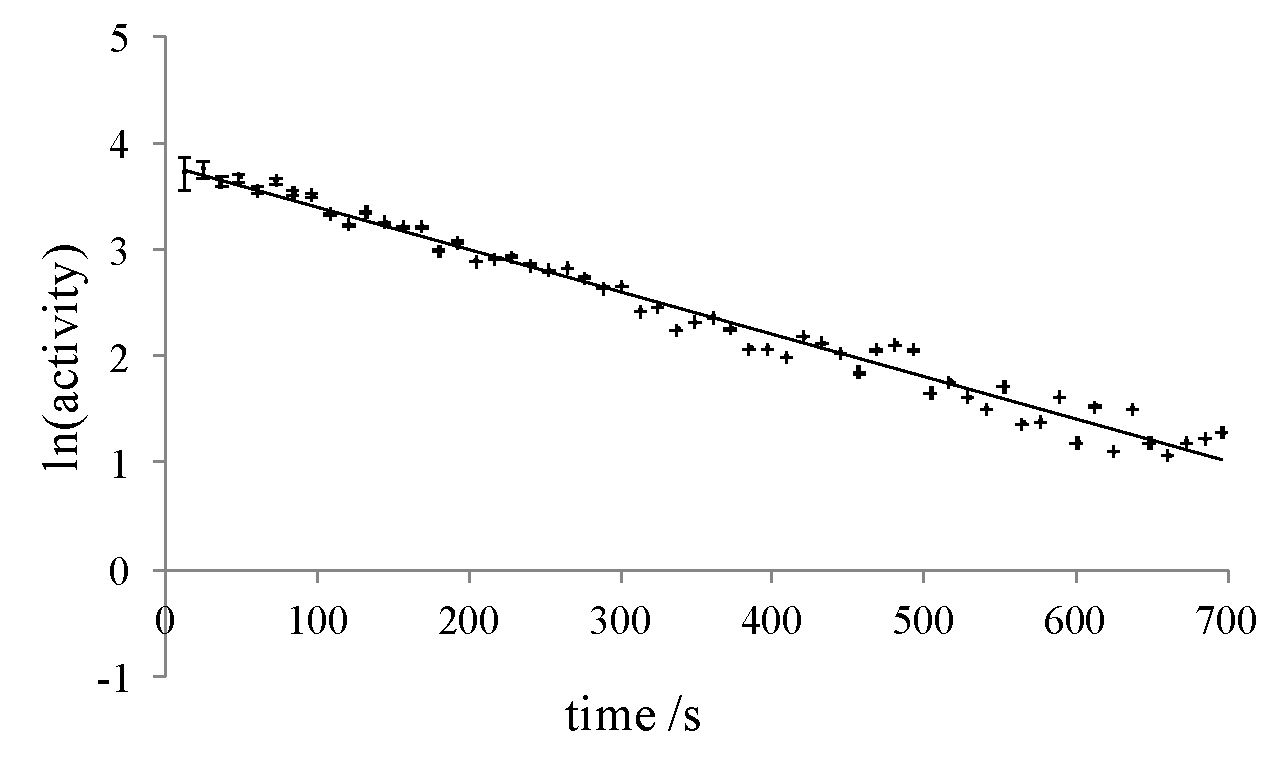
\includegraphics[width=8cm]{fig1}
\caption[]{The natural logarithm of the radioactive activity plotted as a function of time. The vertical error bars are displayed while the horizontal error bars are too small to be seen.}
\label{fig:fig1}
\end{center}
\end{figure}
\squeezeup

The data for the probabilities is plotted onto the same graph, Fig. 2.. It is difficult to distinguish between the Gaussian and Poisson points, they both share a similar distribution as seen by the graph. In terms of the experiment, it would appear that both would be good theoretical models to fit the data by. The mean value of the number of counts is large enough so that the Poisson distribution looks like the Gaussian, there is no particular difference between the two as they both agree with each other. 

On the other hand the experimental probability does not entirely match the theoretical distributions. It bears some resemblance but not completely. The potential reason for this could be due to the lack of data, the experiment was not complete so we cannot make any adequate comparisons between this probability and the theory. We would not be able to discuss on any actual basis how the obtained results would improve if measuring time is increased. 

\begin{figure}[!h]
\begin{center}
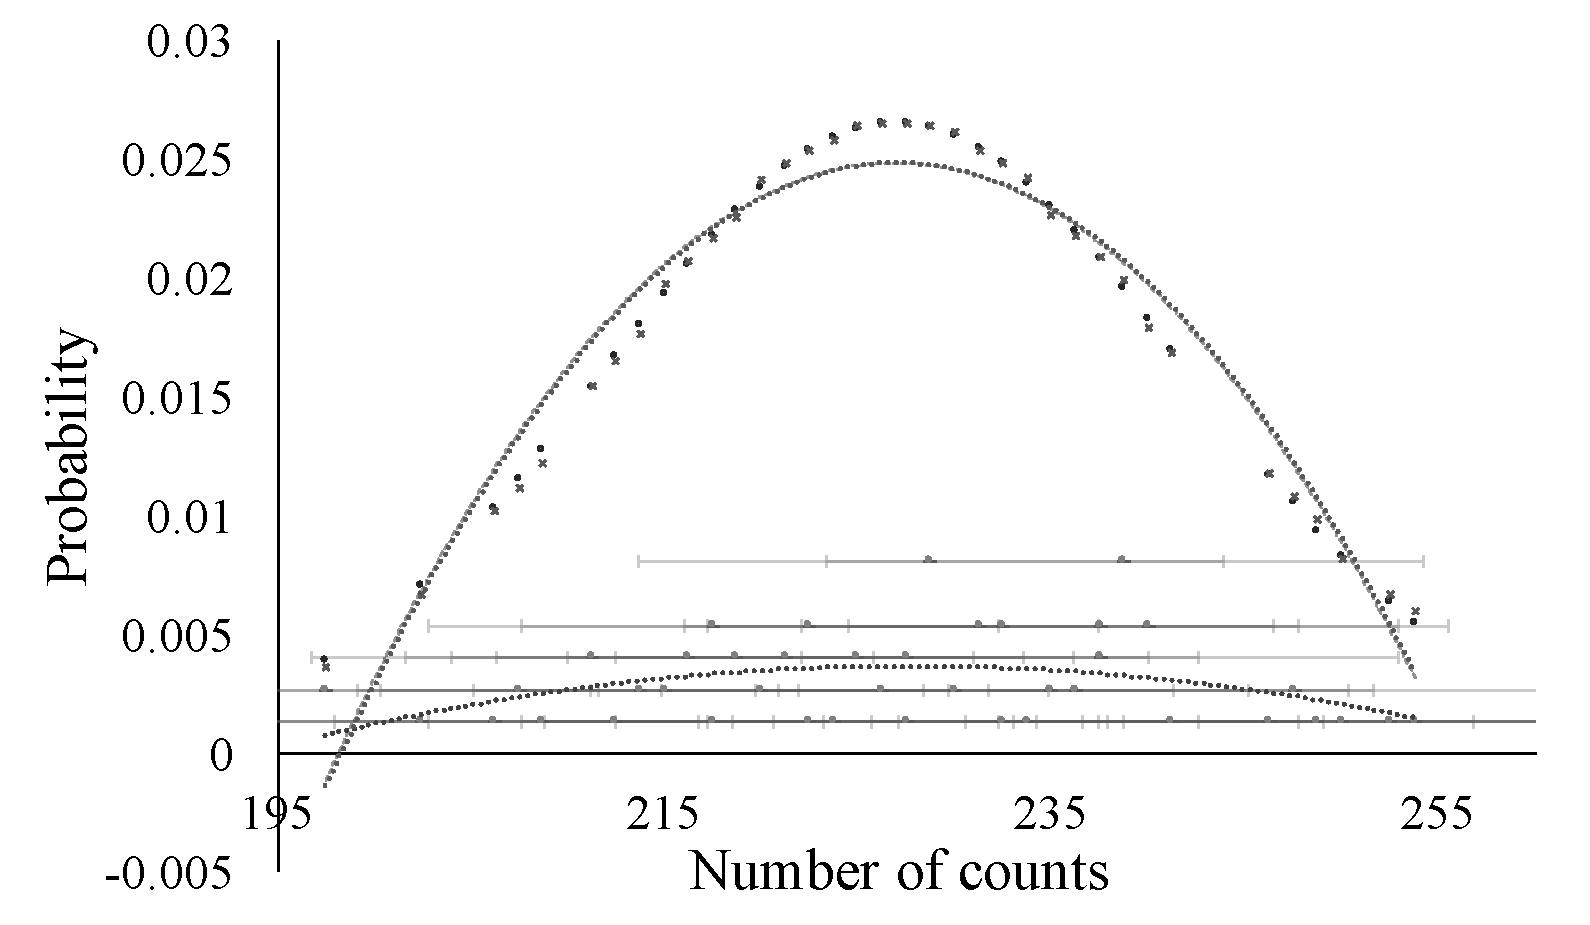
\includegraphics[width=8cm]{fig2}
\caption[]{The experimental (bottom set of points), Poisson (lighter coloured crosses) and Gaussian (darker coloured dots) probabilities plotted with the number of counts.}
\label{fig:fig2}
\end{center}
\end{figure}
\squeezeup
\squeezeup
\squeezeup

It is worth noting the large uncertainty on the number of counts as shown in Fig. 2., the error is about 7\% of the actual value. One possible reason for this could be due to the fact that the data is being applied to a Poisson model and the model does not entirely fit. Or it could be related to the issue above, there is not enough data to provide an adequate result.  

\vspace{-2ex}
\section{Conclusions}
\vspace{-2ex}
 
In conclusion, through experimentation it has been possible to calculate multiple values of half-life for Ba-137m, $t\textsubscript{1/2-CSY}=2.73\pm0.03$ mins and $t\textsubscript{1/2-EXL}=2.92\pm0.07$ mins, values which are similar to the literary value. It has also been possible to construct theoretical probability distributions for random radioactive decay, however comparisons with the experimental probability is not possible as the data set is incomplete. Given more time the experiment could potentially be repeated and then the data could possibly be fitted to the theory, for now that cannot be done. 

\begin{thebibliography}{5}
\bibitem{decay} 
Hugh D. Young and Roger A. Freedman.
\textit{University Physics with Modern Physics, 13th Edition}. 
Pearson Education Limited, Harlow, Essex, 2015.

\bibitem{true} 
W. M. Haynes.
\textit{CRC Handbook of Chemistry and Physics}. 
CRC Press, Florida, USA, 2011.
\end{thebibliography}

\clearpage

\vspace{-3ex}
\section*{Appendix}
\vspace{-2ex}

The uncertainty calculated for $t\textsubscript{1/2-CSY}$ is the standard error, $\alpha_\sigma$. This error only depends on the standard deviation, $\sigma$, and the number of initial half-lives measured $x$,

\begin{equation} \tag{5}
\alpha_\sigma=\sigma \frac{1}{\sqrt{x}}
\end{equation}

 it does not take into account any potential uncertainty on the recorded activity or time period. The precision of the value could have been increased if the number of measurements used to calculate the mean was increased from three to a higher value.
\\

For $t_{1/2-EXL}$ the error, $\alpha_{1/2-EXL}$, is found by using,

\begin{equation} \tag{6}
\alpha_{1/2-EXL}=t_{1/2-EXL}\sqrt{\Big(\frac{\alpha_\lambda}{\lambda}\Big)^2} 
\end{equation}

where $t_{1/2-EXL}$ is the calculated value of half-life from the rearranged equation (2), the value of the decay constant ($\lambda$) was calculated using the LINEST function in Excel, subsequently the error on the decay constant ($\alpha_{\lambda}$) was found by using LINEST as well. 
\\

The uncertainty on $\ln{activity}$ as shown in Fig. 1. was calculated through using the number of counts ($N$), and the time at which the number of counts correspond to ($t$),

\begin{equation} \tag{7}
\alpha_{\ln{A}}=\frac{\sqrt{N}}{12t}
\end{equation}

In measuring the distance between the Am-241 source and the Geiger-M\"{u}ller tube a 30 cm ruler was used, the error here should not matter too much as we do not require it in any of our calculations. However we should at least make a note of it. So, we shall take a value of half of the smallest unit that the ruler can measure to be the uncertainty thus the distance is ($3.0\pm0.5$) cm.

There are no uncertainties for the experimental, Poisson or Gaussian probabilities, but there is uncertainty on the the number of counts measured, $N$. 

\begin{equation} \tag{8}
\alpha_{N}=\sqrt{N}
\end{equation}

This data can have the Poisson distribution applied to it due to the events being random, individual from each other, and occuring over a mean rate without changing.   

%\footnotetext{I am not entirely too sure about what I did for (7), it was help from other students and the demonstrator}

\end{document}